\section{Graphical Models}
\label{sec:graphical-models}

\subsection{Introduction to graphical models}
Remember our goal is to specify the joint distribution \textit{N} random variables $p(x_1,\cdots,x_N)=p(x)$. If we assume each $x_i$ is binary such that $x_i\in\{0,\:1\}$, then we need $\mathbf{2^N-1}$ parameters to specify $p(x)$. For example, $p(x_1=0,\:x_2=0,\:\cdots,x_N=0)\:\text{or}\:p(x_1=1,\:x_2=0,\:\cdots,x_N=0)$.\\ Equivalently, we can specify the joint distribution $p(x)$ as:
\begin{align*}
    p\left(x_1, x_2, \ldots, x_N\right)&=\prod_{j=1}^N p\left(x_j \mid x_1, x_2, \ldots, x_{j-1}\right)\\
    &=p(x_1|x_0)p(x_2|x_1,\:x_0)\cdots
\end{align*}
Thus total number of parameters is $1+2+4+\cdots2^{N-1}=2^N-1$\\
We can see that it requires a huge number of parameters to specify the joint distribution. We want to draw relationships between variables.
\subsubsection*{Condition independence}
For three random variables $x_A,\:x_B\:x_C$, if $x_A,\:x_B$ are conditionally independent given $x_C$, then we write $x_A\perp x_B\mid x_C$. The following conditions are equivalent:
\begin{itemize}
    \item $x_A\perp x_B\mid x_C$
    \item $p(x_A,\:x_B|x_C)=p(x_A|x_C)p(x_B|x_C)$
    \item $p(x_A|x_B,\:x_C)=p(x_A|x_C)$
    \item $p(x_B|x_A,\:x_C)=p(x_B|x_C)$
\end{itemize}
\subsection{Directed Acyclic Graphical Models}
A directed cyclic graphical model encode a particular form of factorization of the joint distribution. The form of factorization is various.\\
\begin{figure}
    \centering
    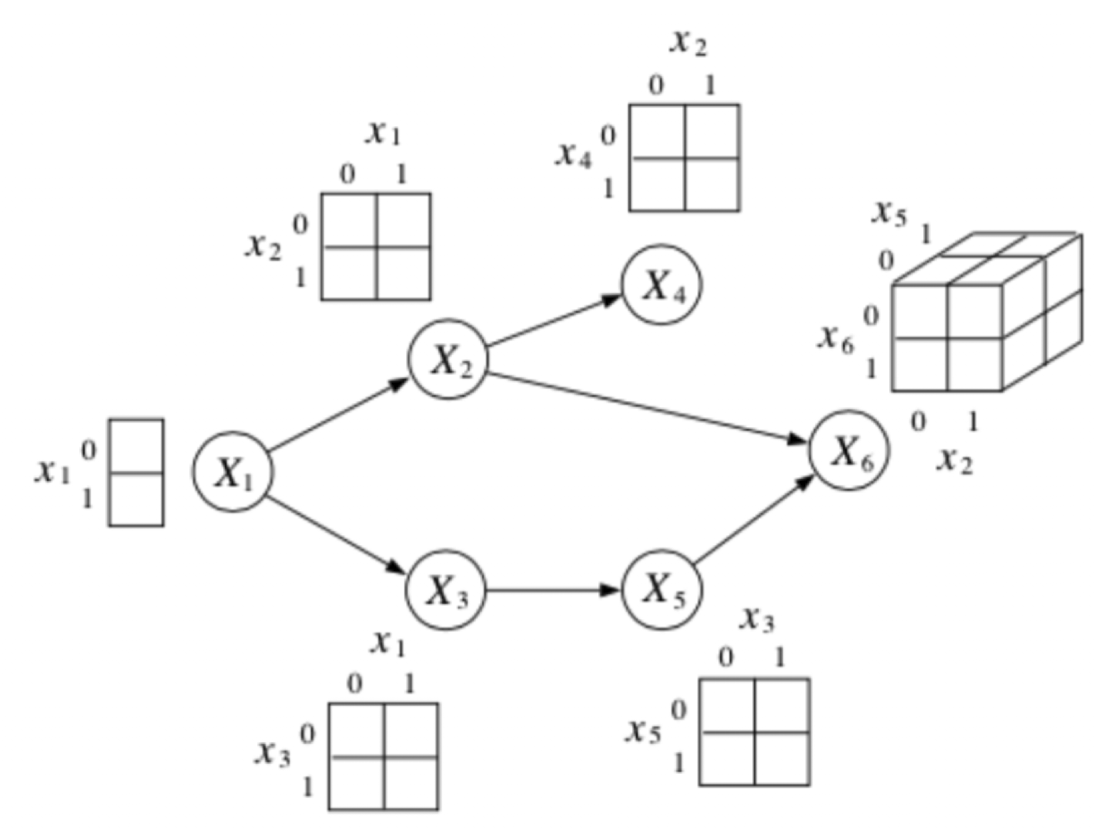
\includegraphics[width=.7\linewidth]{figures/section2/figure_2_1.png}
    \caption{An example of conditional probability tables(CPT)}
    \label{fig:figure_2}
\end{figure}
\hyperref[fig:figure_2]{Figure 2} shows an example of conditional probability. From the graph, we only need $2^1*4+2^0+2^2=13<2^6-1$ parameters.\\
\textbf{D-separation}: If $C$ d-separates $A$ and $B$, then $x_A\perp x_B\mid x_C\:\forall a\in A,\:b\in B$
\subsubsection*{Bayes ball algorithm}
Bayes ball determines the conditional independence/dependence in a DAG (I personally found this part most ambiguous). There are three fundamental Bayes ball algorithms which are causal chain, common cause and explaining away. For each one, we will under it intuitively by drawing a story.
\begin{enumerate}
  \item \textbf{Causal chain}

  \begin{figure}[H]
    \centering
    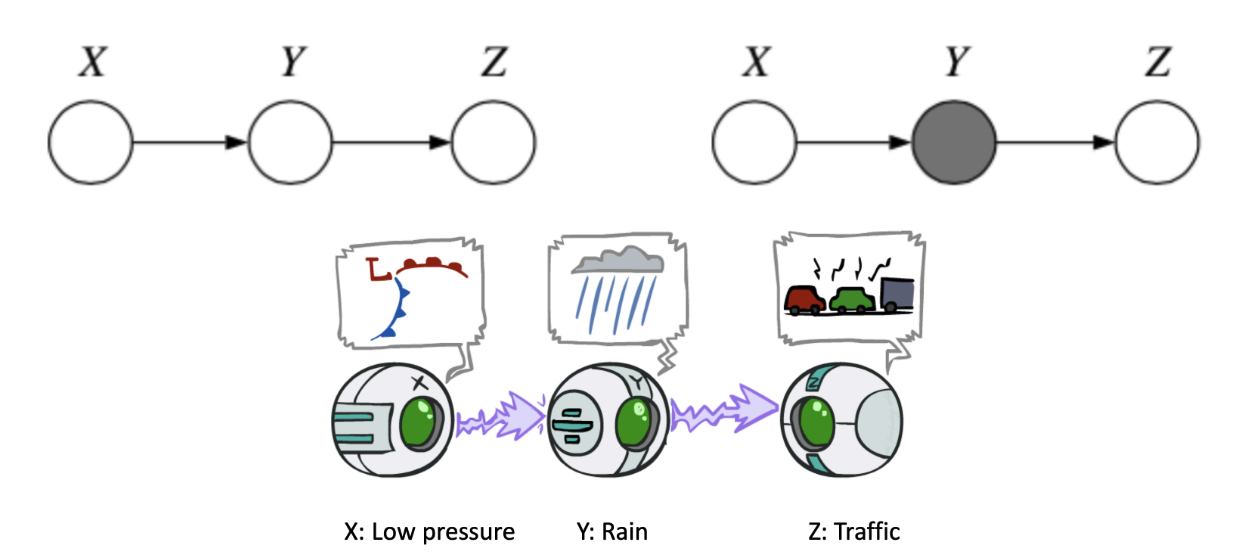
\includegraphics[width = .7\linewidth]{figures/section2/figure_2_2.png}
    \caption{An illustration of causal chain}
  \end{figure}
  \begin{align*}
    p(z \mid x, y) & =\frac{p(x, y, z)}{p(x, y)} \\
    & =\frac{p(x) p(y \mid x) p(z \mid y)}{p(x) p(y \mid x)} \\
    & =p(z \mid y) \quad \\
    \Rightarrow X\text { and }& Z \text { d-separated given } Y
  \end{align*}
  
  \item \textbf{Common cause}

  \begin{figure}[H]
    \centering
    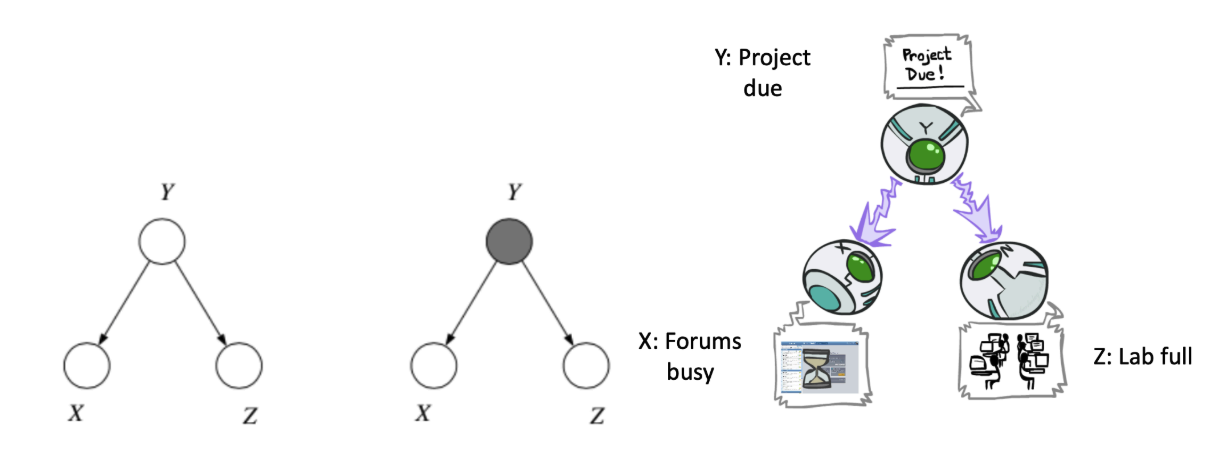
\includegraphics[width = .7\linewidth]{figures/section2/figure_2_3.png}
    \caption{An illustration of common cause}
  \end{figure}
  \begin{align*}
    p(x, z \mid y)&=\frac{p(x, y, z)}{p(y)}\\
    &=\frac{p(y) p(x \mid y) p(z \mid y)}{p(y)}\\
    &=p(x \mid y) p(z \mid y)\\
    \Rightarrow X\text { and }& Z \text { d-separated given } Y
  \end{align*}
  
  \item \textbf{Explaining away}

  \begin{figure}[H]
    \centering
    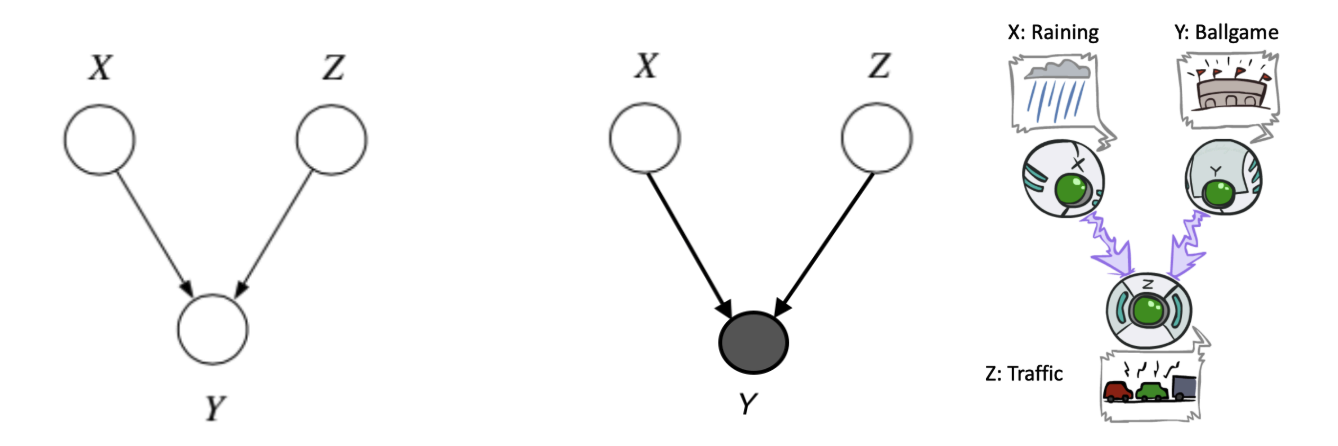
\includegraphics[width = .7\linewidth]{figures/section2/figure_2_4.png}
    \caption{An illustration of explaining away}
  \end{figure}
  \begin{align*}
    p(z \mid x, y) & =\frac{p(x) p(z) p(y \mid x, z)}{p(x) p(y \mid x)} \\
    & =\frac{p(z) p(y \mid x, z)}{p(y \mid x)} \neq p(z \mid y)\\
    \Rightarrow X\text { and }& Z \text { are NOT d-separated given } Y
  \end{align*}
\end{enumerate}
In general, the Bayes ball works as follows:
\begin{enumerate}
    \item Shade all nodes $x_C$ (these are observed)
    \item Place "balls" at each node in $x_A$ (or $x_B$ )
    \item Let the "balls" "bounce" around according to some rules. If any of the balls reach any of the nodes in $x_B$ from $x_A$ then $x_A \not\perp x_B \mid x_C$. Otherwise $x_A \perp x_B \mid x_C$
\end{enumerate}
\textbf{Example}\\
\textit{Question:} Is $x_2\perp x_3\mid\{x_1,\:x_6\}$
\begin{figure}[H]
    \centering
    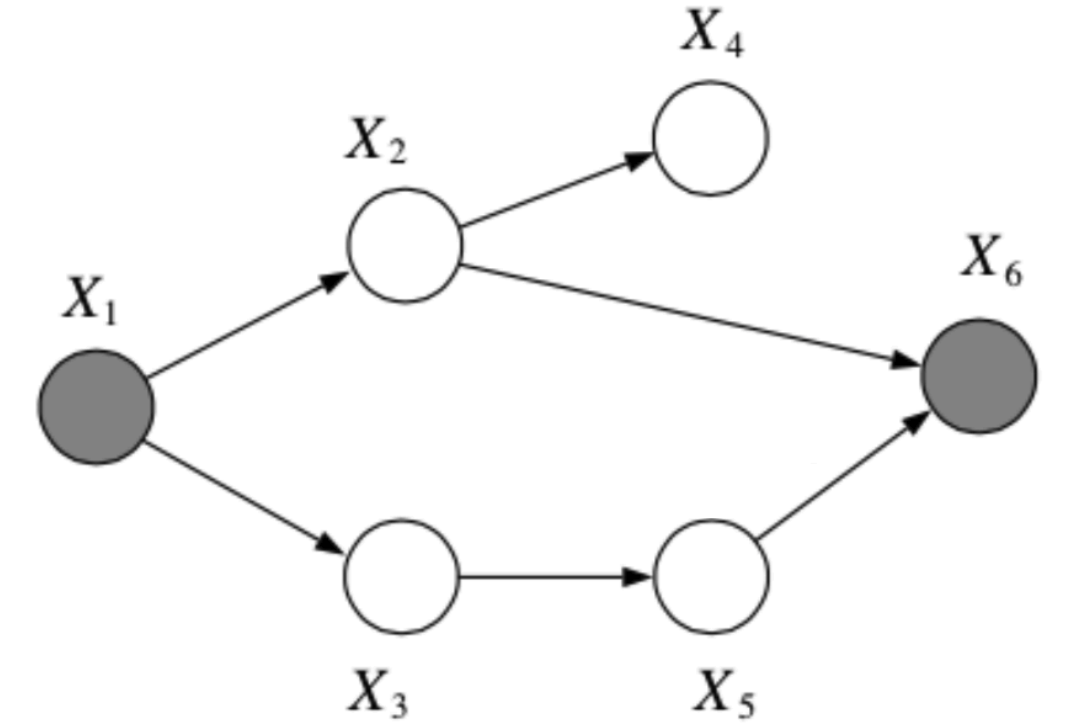
\includegraphics[width = .7\linewidth]{figures/section2/figure_2_5.png}
    \caption{An illustration of explaining away}
  \end{figure}
\textit{Answer:} No. By Bayes ball algorithm, $x_2$ can travel to $x_5$, and hence can travel to $x_3$.
\subsubsection*{Moralization}
Like I said, I personally do not like Bayes algorithm. Instead, another one called "moralization" is more straightforward and easier to use. We can follow the procedure:
\begin{enumerate}
    \item \textbf{Draw the ancestral graph}\\
    We only keep the ancestor of the mentioned nodes. That said, in the previous example, we only keep the ancestors of $\{x_2,\:x_3,\:x_1\:x_6\}$. Hence we have the entire graph except the node $x_4$. Note the ancestors includes \textbf{their parents, parents' parents etc}.
    \item \textbf{"Moralize" the ancestral graph by "marrying" the parents}\\
    If two nodes have the same children, such as $x_2$ and $x_5$, then we draw a line between these two nodes.
    \item \textbf{"Disorient" the graph}\\
    Ignore the directions by replacing the arrows to edges.
    \item \textbf{Delete the givens and their edges}\\
    In the previous example, the givens are the $x_1$ and $x_4$.
    \item \textbf{Find the answer}\\
    After we finished the step 1 to 4, we then justify whether the two nodes are connected or disconnected. If \textbf{connected}, then the two nodes are conditionally \textbf{dependent}. Otherwise \textbf{disconnected}, the two nodes are conditionally \textbf{independent}. In the previous example, we can easily find that $x_2$ and $x_3$ are d-separated by $x_1$ and $x_6$.
\end{enumerate}
\textit{Question}: What about the marginal independence, such as $x_2\perp x_3$?\\
\textit{Answer}: We use the same way as above without step 4.

\subsection{Undirected Graphical Models}
The undirected graphical models are also called the \textbf{Markov random fields (MRFs)}. Compare to graphical models, we have no more directed edges; instead, the dependencies are now described as undirected graphs. Moreover, \textbf{Markov blanket} is the set of nodes that makes $X_i$ conditionally independent of all other nodes. \textbf{Clique} is a subset of nodes that every two nodes are connected by an edge. \textbf{Maximal clique} a clique that can not be extended by including one more adjacent vertex.
\begin{figure}[H]
    \centering
    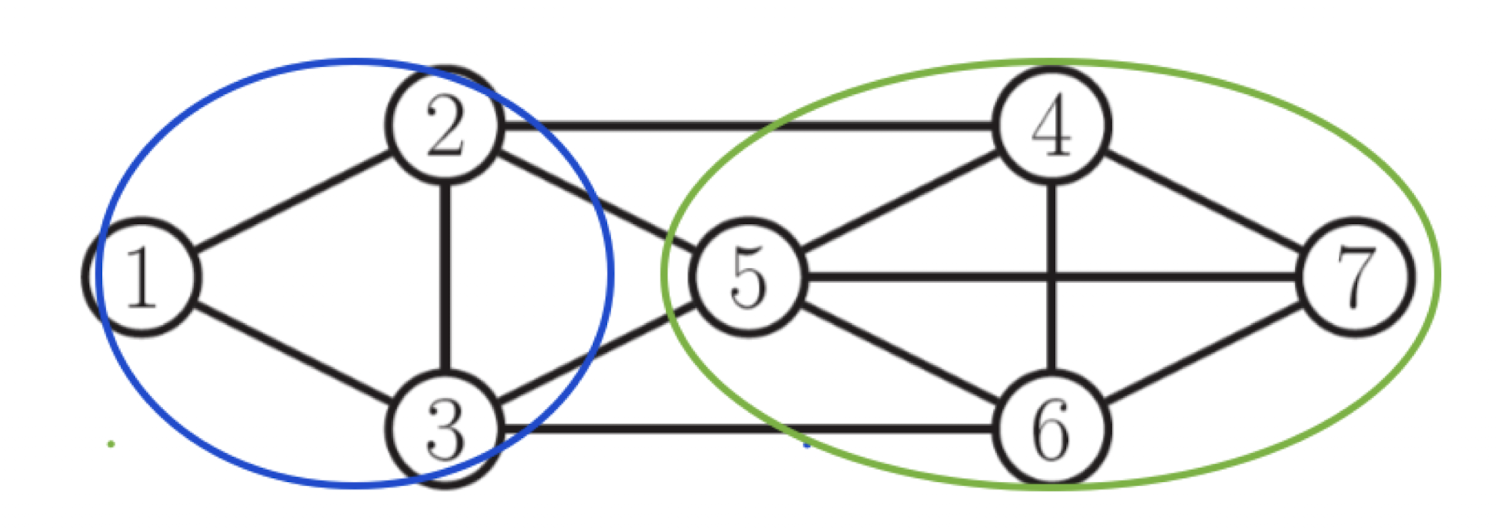
\includegraphics[width = .7\linewidth]{figures/section2/figure_2_6.png}
    \caption{An example of Markov random fields: \{1, 2, 3\} is a clique and \{4, 5, 6, 7\} is a maximal clique}
    \label{fig:mrf}
\end{figure}
\subsubsection*{Distribution induced by MRFs}
\begin{itemize}
    \item Let $X=\left(X_1, \ldots, X_m\right)$ be the set of all random variables in our graph $G$.
    \item Let $\mathcal{C}$ be the set of all maximal cliques of $G$.
    \item The distribution $p$ of $X$ factorizes with respect to $G$ if
$$
p(x) \propto \prod_{C \in \mathcal{C}} \psi_{\mathcal{C}}\left(x_C\right)
$$
for some nonnegative potential functions $\psi_C$, where $x_C=\left(x_i\right)_{i \in C}$.
\end{itemize}
The density can be factorized to cliques is also called the \textbf{Hammersley-Clifford Theorem}.\\
\textbf{Global markov properties}: $X_A\perp X_B\mid X_S$ if the sets $A$ and $B$ are separated by $S$ in $G$ (every path from $A$ to $B$ has to pass $S$).
Therefore, the joint distribution described on \hyperlink{fig:mrf}{above} is: 
\begin{align*}
  p(x) \propto & \psi_{1,2,3}\left(x_1, x_2, x_3\right) \psi_{2,3,5}\left(x_2, x_3, x_5\right) \psi_{2,4,5}\left(x_2, x_4, x_5\right) \\
  & \times \psi_{3,5,6}\left(x_3, x_5, x_6\right) \psi_{4,5,6,7}\left(x_4, x_5, x_6, x_7\right)
  \end{align*}
\colorbox{yellow}{Not all DAGMs can be represented as MRFs.}.\\
\subsubsection*{Relations between exponential families and MRFs}
\begin{itemize}
  \item Consider a parametric family of factorized distributions
  $$
  p(x \mid \theta)=\frac{1}{Z(\theta)} \prod_{C \in \mathcal{C}} \psi_c\left(x_C \mid \theta_C\right), \quad \theta=\left(\theta_C\right)_{c \in \mathcal{C}} .
  $$
  \item We can write this in an exponential form:
  $$
  p(x \mid \theta)=\exp \{\sum_{C \in \mathcal{C}} \log \psi_C\left(x_C \mid \theta_C\right)-\underbrace{\log Z(\theta)}_{=A(\theta)}\}
  $$
  \item Suppose the potentials have a log-linear form
  $$
  \log \psi_C\left(x_C \mid \theta_C\right)=\theta_C^{\top} \phi_C\left(x_C\right)
  $$
  we then get the exponential family
  $$
  p(x \mid \theta)=\exp \{\sum_{C \in \mathcal{C}} \theta_C^{\top} \phi_C\left(x_C\right)-\underbrace{\log Z(\theta)}_{=A(\theta)}\}
  $$
\end{itemize}
\textit{Question}: When the potentials have a log-linear form?\\
\textit{Solution}: Suppose we have the random vector $x_1$ and $x_2$, and they are all binary. Then there are four possible values of $(x_1,\:x_2)$: (0, 0), (1, 0), (0, 1), (1, 1). We take\\
$$
\theta_{1,2}:=\left[\begin{array}{l}
\log \psi_{1,2}(0,0) \\
\log \psi_{1,2}(0,1) \\
\log \psi_{1,2}(1,0) \\
\log \psi_{1,2}(1,1)
\end{array}\right] \in \mathbb{R}^4
$$
and let $\psi_{1,2}\left(x_1, x_2\right)$ be the function that satisfies
$$
\phi_{1,2}(0,0)=\left[\begin{array}{l}
1 \\
0 \\
0 \\
0
\end{array}\right], \quad \phi_{1,2}(0,1)=\left[\begin{array}{l}
0 \\
1 \\
0 \\
0
\end{array}\right], \quad \phi_{1,2}(1,0)=\left[\begin{array}{l}
0 \\
0 \\
1 \\
0
\end{array}\right], \quad \phi_{1,2}(1,1)=\left[\begin{array}{l}
0 \\
0 \\
0 \\
1
\end{array}\right].
$$

$$\Rightarrow\phi_{1,2}\left(x_1, x_2\right)=\left[\begin{array}{c}
  \left(1-x_1\right)\left(1-x_2\right) \\
  \left(1-x_1\right) x_2 \\
  x_1\left(1-x_2\right) \\
  x_1 x_2
  \end{array}\right]
$$
We then have a linear form:$$
\log \psi_C\left(x_{12} \mid \theta_{12}\right)=\theta_{12}^{\top} \phi_{12}\left(x_{12}\right)
$$
\subsubsection*{Ising model}
The Ising model is an example of MRFs, which is used to model magnets. It has a form of potential function:
$$\psi_{st}(x_s,\:x_t)=e^{J_{st}x_sx_t}$$
Equivalently:
$$\psi_{st}(-1,\:-1)=\psi_{st}(1,\:1)=e^{J_{st}}$$
$$\psi_{st}(1,\:-1)=\psi_{st}(-1,\:1)=e^{-J_{st}}$$
$$\psi_{st}(x_s,\:x_t)=0\:\text{if the two nodes are not connected}$$
In terms of the distribution in Ising model, we also incldue the node potential $\psi_s(x_s)=e^{b_sx_s}$:
$$p(x) \propto \prod_{s \sim t} \psi_{s t}\left(x_s, x_s\right) \prod_s \psi_s\left(x_s\right)=\exp \left\{\sum_{s \sim t} J_{s t} x_s x_t+\sum_s b_s x_s\right\}$$
\textbf{Recall: Multivariate normal distribution}\\
$X=\left(X_1, \ldots, X_m\right): \mu \in \mathbb{R}^m$ and $\Sigma$ symmetric positive definite $m \times m$ matrix. Write $X \sim N_m(\mu, \Sigma)$ if the density of the vector $X$ is
$$
f(\boldsymbol{x} ; \mu, \Sigma)=\frac{1}{(2 \pi)^{m / 2}}(\operatorname{det} \Sigma)^{-1 / 2} \exp \left(-\frac{1}{2}(\boldsymbol{x}-\mu)^T \Sigma^{-1}(\boldsymbol{x}-\mu)\right) .
$$
Denote $K=\Sigma^{-1}$ then
$$
f(\boldsymbol{x} ; \mu, \Sigma) \propto \prod_{\boldsymbol{s}} e^{-\frac{1}{2} K_{s s}\left(x_s-\mu_s\right)^2} \prod_{\boldsymbol{s}<t} e^{-K_{s t}\left(x_s-\mu_s\right)\left(x_t-\mu_t\right)}
$$
Intuitively, we can also visualize the conditional independencies between each variables (similar to Bayes ball). Just like the Ising model, here we can use concentration matrix $K$ to represent the relationship between variables.\\
Conditional independence:
\begin{itemize}
  \item $X_i \perp X_j$ if and only if $\Sigma_{i j}=0$.
  \item $X_i \perp X_j \mid X_C \quad$ if and only if $\quad \Sigma_{i j}-\Sigma_{i, C} \Sigma_{C, C}^{-1} \Sigma_{C, j}=0$
  \item Let $R=V \backslash\{i, j\}$. The following are equivalent:
  \begin{itemize}
    \item $X_i \perp X_j \mid X_R$
  \item $\Sigma_{i j}-\Sigma_{i, R} \Sigma_{R, R}^{-1} \Sigma_{R, j}=0$
  \item $\left(\Sigma^{-1}\right)_{i j}=0$ 
  \end{itemize}
\end{itemize}
Hence we have the \textbf{Gaussian Graphical models}
\begin{figure}[H]
  \centering
  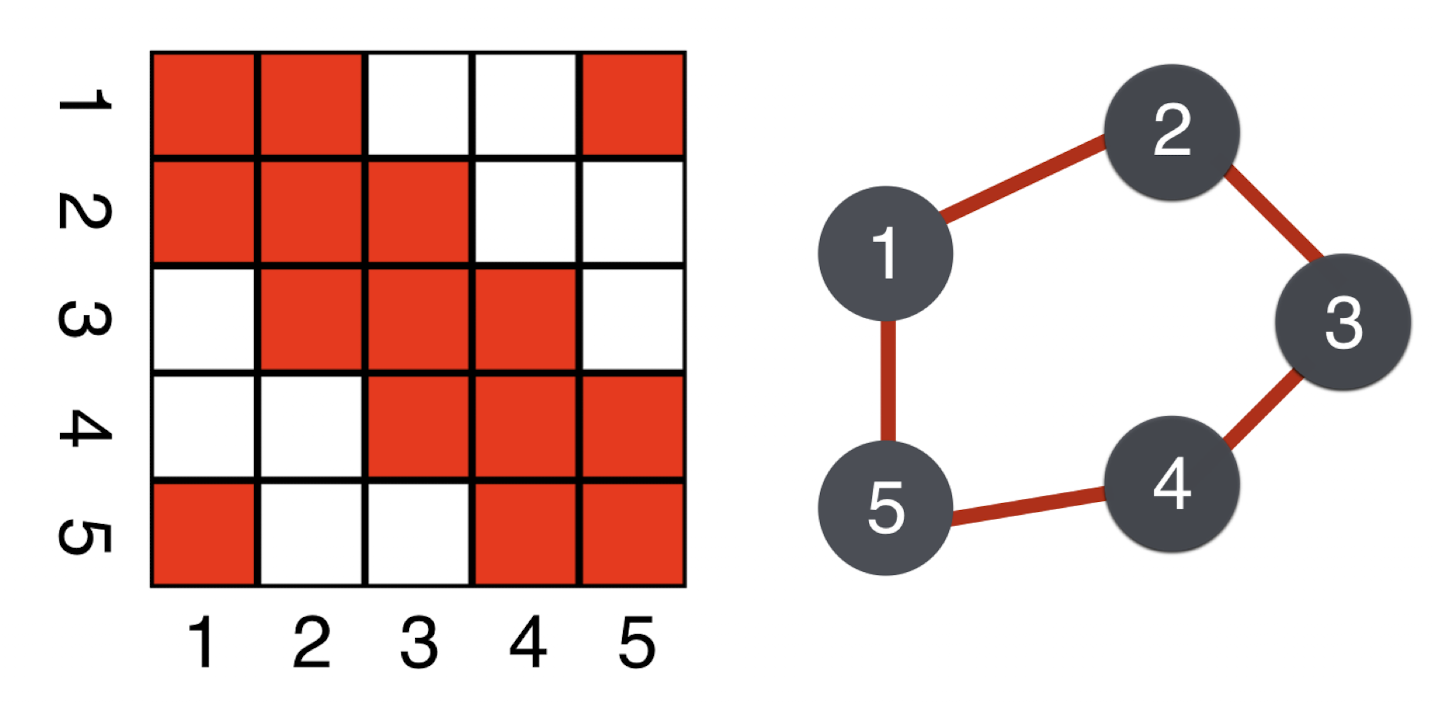
\includegraphics[width = .7\linewidth]{figures/section2/figure_2_7.png}
  \caption{An example of Gaussian Graphical model}
  \label{fig:ggm}
\end{figure}
$K_{ij}=0$ if and only if $X_i\perp X_j\mid X_{rest}$. For example, $X_1\perp X_4\mid X_{rest}$